\documentclass[11pt,a4paper]{article}
\newcommand{\intestazione}{Trimero ad anello --- 11. Readout asimmetrico}
% =====================================================================
%  Preambolo comune ai documenti sul dimero (serie "che cosa abbiamo fatto")
%  Incluso con % =====================================================================
%  Preambolo comune ai documenti sul dimero (serie "che cosa abbiamo fatto")
%  Incluso con % =====================================================================
%  Preambolo comune ai documenti sul dimero (serie "che cosa abbiamo fatto")
%  Incluso con \input{preambolo_dimero} subito dopo \documentclass.
% =====================================================================
\usepackage[T1]{fontenc}
\usepackage[utf8]{inputenc}
\usepackage[main=italian,provide=*]{babel}
\usepackage{amsmath,amssymb,mathtools}
\usepackage{graphicx}
\usepackage{booktabs}
\usepackage{colortbl}
\usepackage{xcolor}
\usepackage{geometry}
\usepackage{placeins}
\usepackage{caption}
\usepackage{enumitem}
\usepackage{fancyhdr}
\usepackage{needspace}
\usepackage{tikz}
\usetikzlibrary{arrows.meta,positioning,shapes.geometric,calc,fit,backgrounds}
\usepackage{hyperref}
\hypersetup{colorlinks=true,linkcolor=blu,citecolor=blu,urlcolor=blu}

\geometry{margin=2.5cm}

% --- colori coerenti con quelli delle figure (palette Okabe-Ito)
\definecolor{blu}{HTML}{0072B2}
\definecolor{arancio}{HTML}{E69F00}
\definecolor{verdes}{HTML}{009E73}
\definecolor{rossos}{HTML}{D55E00}
\definecolor{violas}{HTML}{CC79A7}
\definecolor{grigetto}{HTML}{E8E8E8}

\captionsetup{font=small,labelfont=bf,width=0.92\textwidth}

\pagestyle{fancy}
\fancyhf{}
\fancyhead[L]{\small\itshape\intestazione}
\fancyhead[R]{\small\thepage}
\renewcommand{\headrulewidth}{0.3pt}

% --- notazione
\newcommand{\ket}[1]{\lvert #1\rangle}
\newcommand{\bra}[1]{\langle #1 \rvert}
\newcommand{\media}[1]{\langle #1 \rangle}
\newcommand{\vs}[1]{\mathbf{s}_{#1}}

% --- riquadro "in una riga": il messaggio da portare a casa
\newcommand{\messaggio}[1]{%
  \begin{center}
  \begin{minipage}{0.93\textwidth}
  \setlength{\fboxsep}{9pt}%
  \colorbox{grigetto}{\begin{minipage}{\dimexpr\textwidth-2\fboxsep}
  \small\textbf{In una riga.}\enspace #1
  \end{minipage}}
  \end{minipage}
  \end{center}
}

% --- riquadro "come lo sappiamo": la verifica numerica dietro un'affermazione
\newcommand{\verifica}[1]{%
  \begin{center}
  \begin{minipage}{0.93\textwidth}
  \small\textcolor{verdes}{\rule{2.2em}{1.1pt}}\enspace
  \textcolor{verdes}{\textbf{Come lo sappiamo.}}\enspace #1
  \end{minipage}
  \end{center}
  \medskip
}
 subito dopo \documentclass.
% =====================================================================
\usepackage[T1]{fontenc}
\usepackage[utf8]{inputenc}
\usepackage[main=italian,provide=*]{babel}
\usepackage{amsmath,amssymb,mathtools}
\usepackage{graphicx}
\usepackage{booktabs}
\usepackage{colortbl}
\usepackage{xcolor}
\usepackage{geometry}
\usepackage{placeins}
\usepackage{caption}
\usepackage{enumitem}
\usepackage{fancyhdr}
\usepackage{needspace}
\usepackage{tikz}
\usetikzlibrary{arrows.meta,positioning,shapes.geometric,calc,fit,backgrounds}
\usepackage{hyperref}
\hypersetup{colorlinks=true,linkcolor=blu,citecolor=blu,urlcolor=blu}

\geometry{margin=2.5cm}

% --- colori coerenti con quelli delle figure (palette Okabe-Ito)
\definecolor{blu}{HTML}{0072B2}
\definecolor{arancio}{HTML}{E69F00}
\definecolor{verdes}{HTML}{009E73}
\definecolor{rossos}{HTML}{D55E00}
\definecolor{violas}{HTML}{CC79A7}
\definecolor{grigetto}{HTML}{E8E8E8}

\captionsetup{font=small,labelfont=bf,width=0.92\textwidth}

\pagestyle{fancy}
\fancyhf{}
\fancyhead[L]{\small\itshape\intestazione}
\fancyhead[R]{\small\thepage}
\renewcommand{\headrulewidth}{0.3pt}

% --- notazione
\newcommand{\ket}[1]{\lvert #1\rangle}
\newcommand{\bra}[1]{\langle #1 \rvert}
\newcommand{\media}[1]{\langle #1 \rangle}
\newcommand{\vs}[1]{\mathbf{s}_{#1}}

% --- riquadro "in una riga": il messaggio da portare a casa
\newcommand{\messaggio}[1]{%
  \begin{center}
  \begin{minipage}{0.93\textwidth}
  \setlength{\fboxsep}{9pt}%
  \colorbox{grigetto}{\begin{minipage}{\dimexpr\textwidth-2\fboxsep}
  \small\textbf{In una riga.}\enspace #1
  \end{minipage}}
  \end{minipage}
  \end{center}
}

% --- riquadro "come lo sappiamo": la verifica numerica dietro un'affermazione
\newcommand{\verifica}[1]{%
  \begin{center}
  \begin{minipage}{0.93\textwidth}
  \small\textcolor{verdes}{\rule{2.2em}{1.1pt}}\enspace
  \textcolor{verdes}{\textbf{Come lo sappiamo.}}\enspace #1
  \end{minipage}
  \end{center}
  \medskip
}
 subito dopo \documentclass.
% =====================================================================
\usepackage[T1]{fontenc}
\usepackage[utf8]{inputenc}
\usepackage[main=italian,provide=*]{babel}
\usepackage{amsmath,amssymb,mathtools}
\usepackage{graphicx}
\usepackage{booktabs}
\usepackage{colortbl}
\usepackage{xcolor}
\usepackage{geometry}
\usepackage{placeins}
\usepackage{caption}
\usepackage{enumitem}
\usepackage{fancyhdr}
\usepackage{needspace}
\usepackage{tikz}
\usetikzlibrary{arrows.meta,positioning,shapes.geometric,calc,fit,backgrounds}
\usepackage{hyperref}
\hypersetup{colorlinks=true,linkcolor=blu,citecolor=blu,urlcolor=blu}

\geometry{margin=2.5cm}

% --- colori coerenti con quelli delle figure (palette Okabe-Ito)
\definecolor{blu}{HTML}{0072B2}
\definecolor{arancio}{HTML}{E69F00}
\definecolor{verdes}{HTML}{009E73}
\definecolor{rossos}{HTML}{D55E00}
\definecolor{violas}{HTML}{CC79A7}
\definecolor{grigetto}{HTML}{E8E8E8}

\captionsetup{font=small,labelfont=bf,width=0.92\textwidth}

\pagestyle{fancy}
\fancyhf{}
\fancyhead[L]{\small\itshape\intestazione}
\fancyhead[R]{\small\thepage}
\renewcommand{\headrulewidth}{0.3pt}

% --- notazione
\newcommand{\ket}[1]{\lvert #1\rangle}
\newcommand{\bra}[1]{\langle #1 \rvert}
\newcommand{\media}[1]{\langle #1 \rangle}
\newcommand{\vs}[1]{\mathbf{s}_{#1}}

% --- riquadro "in una riga": il messaggio da portare a casa
\newcommand{\messaggio}[1]{%
  \begin{center}
  \begin{minipage}{0.93\textwidth}
  \setlength{\fboxsep}{9pt}%
  \colorbox{grigetto}{\begin{minipage}{\dimexpr\textwidth-2\fboxsep}
  \small\textbf{In una riga.}\enspace #1
  \end{minipage}}
  \end{minipage}
  \end{center}
}

% --- riquadro "come lo sappiamo": la verifica numerica dietro un'affermazione
\newcommand{\verifica}[1]{%
  \begin{center}
  \begin{minipage}{0.93\textwidth}
  \small\textcolor{verdes}{\rule{2.2em}{1.1pt}}\enspace
  \textcolor{verdes}{\textbf{Come lo sappiamo.}}\enspace #1
  \end{minipage}
  \end{center}
  \medskip
}


\title{\bfseries Quando la scala moltiplicativa non basta più\\[2pt]
\large Documento 11 --- estensione facoltativa, nessuna sorpresa}
\author{Samuele Schiavi \\ \small Tesi triennale in Fisica, Università di Parma
--- Relatore: Prof.\ Alessandro Chiesa}
\date{}

\begin{document}
\maketitle
\thispagestyle{fancy}

\section{Una domanda lasciata esplicitamente aperta}

Punto di lavoro: \textbf{Scenario A} ($b/J=2.4$, $D/J=0.15$, Opzione DM B),
correlatore $C_{21}^{xx}(t{=}2)$ --- gli stessi dei Documenti 6--10. Il
readout simmetrico ($p_{01}=p_{10}=p$) usato finora è una
semplificazione: su hardware reale il rilassamento $T_1$ durante la misura
rende tipicamente $p_{10}>p_{01}$. Il relatore l'aveva segnalato come
opzionale sul dimero (``parti simmetrico, poi vedi se hai tempo di fare un
test asimmetrico''); qui si ripete lo stesso controllo, con la
metodologia a shot finiti di questa serie.

\section{Perché non è la ripetizione di un conto già chiuso}

Il circuito dei correlatori dell'anello ha un registro più grande di
quello del dimero (tre qubit contro due) --- la domanda naturale è se
questo introduca una complicazione nuova per la correzione di readout.

\verifica{Verificato direttamente dal codice
(\texttt{circuito\_correlazioni\_trimero\_anello.py}): il circuito misura
un solo bit classico, sempre e solo l'ancilla. La correzione di readout
asimmetrico si applica a quella singola misura --- una proprietà del
\emph{numero di bit misurati}, non del numero di qubit di registro. Il
registro più grande non introduce nulla di nuovo.}

\section{Da dove viene l'asimmetria, fisicamente}

Con una matrice di confusione generale, $p_{01}\neq p_{10}$:
$$\langle Z\rangle_\text{readout} = \alpha\langle Z\rangle_\text{ideale}+\beta,
\qquad \alpha=1-p_{01}-p_{10},\ \ \beta=p_{10}-p_{01}.$$
Per il correlatore complesso, una traslazione costante nel piano
complesso --- non garantita a priori preservare l'invarianza di
$N^*=\arg\max_N|C(N)|$ (somma e modulo non commutano), come già verificato
sul dimero.

\section{Un dettaglio verificato prima di scrivere il resto del codice}

Sul dimero l'ancilla è il qubit $0$: con \texttt{measure\_all()} il suo
bit è l'\textbf{ultimo} carattere della stringa di misura. Sull'anello
l'ancilla è il qubit $3$ (convenzione ereditata dalla Parte 1): il suo bit
è il \textbf{primo} carattere.

\verifica{Circuito di controllo: $X$ solo sull'ancilla, registro
$\ket{000}$, 100 shot $\to$ \texttt{\{'1000': 100\}} --- confermato, prima
di fidarsi di qualunque numero successivo.}

\section{I valori scelti, e perché}

Nessuno split reale citabile per \texttt{ibm\_torino} specificamente ---
stessa situazione del dimero. Split illustrativo, identico a quello già
usato lì per confrontabilità diretta: rapporto $p_{10}/p_{01}=3\times$,
stessa media $p_\text{readout}=2.3\times10^{-2}$ ($p_{01}=0.0115$,
$p_{10}=0.0345$).

\section{Risultati: il correlatore, simmetrico contro asimmetrico}

Tutto a shot finiti: nessuna formula analitica, il \texttt{ReadoutError}
asimmetrico agganciato al \texttt{NoiseModel} è l'unico metodo.

\begin{figure}[htbp]
\centering
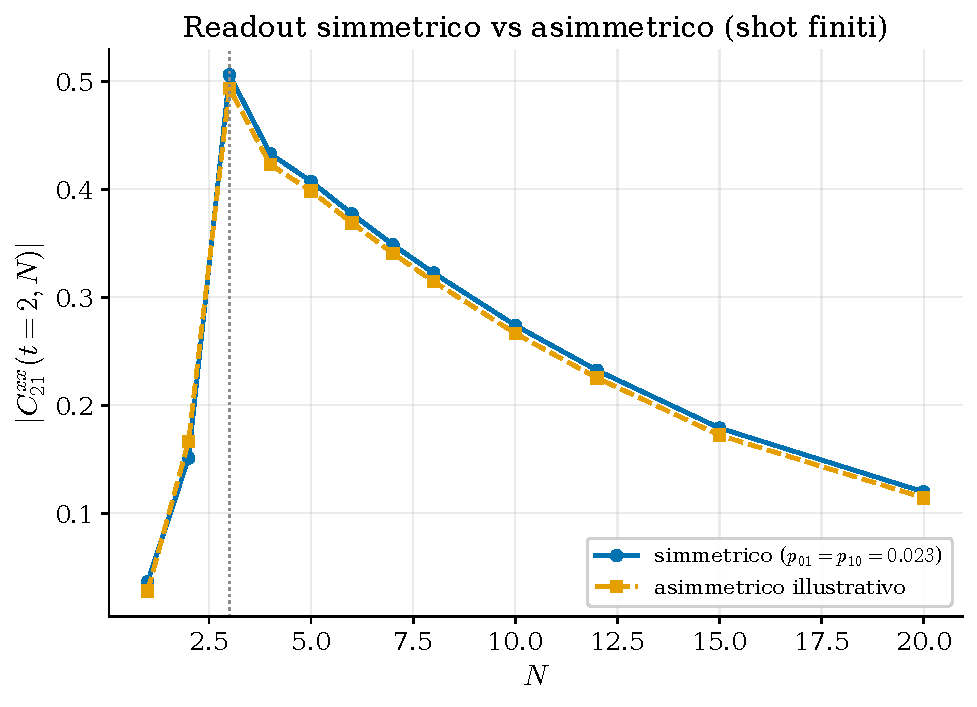
\includegraphics[width=0.72\textwidth]{figure/fig_correlatore_N_asimmetrico_anello}
\caption{$|C_{21}^{xx}(t{=}2,N)|$, readout simmetrico contro asimmetrico
($8\times10^4$ shot per punto). $N^*=3$ in entrambi i casi.}
\end{figure}
\FloatBarrier

\begin{table}[htbp]
\centering
\small
\renewcommand{\arraystretch}{1.3}
\begin{tabular}{@{}lcc@{}}
\toprule
\rowcolor{grigetto}
& $N^*$ & $|C(N^*)|$ \\
\midrule
simmetrico ($p_{01}=p_{10}=0.023$) & 3 & $0.5059$ \\
asimmetrico ($3\times$) & 3 & $0.4934$ \\
\bottomrule
\end{tabular}
\end{table}
\FloatBarrier

\section{Uno stress test oltre il range realistico}

\begin{figure}[htbp]
\centering
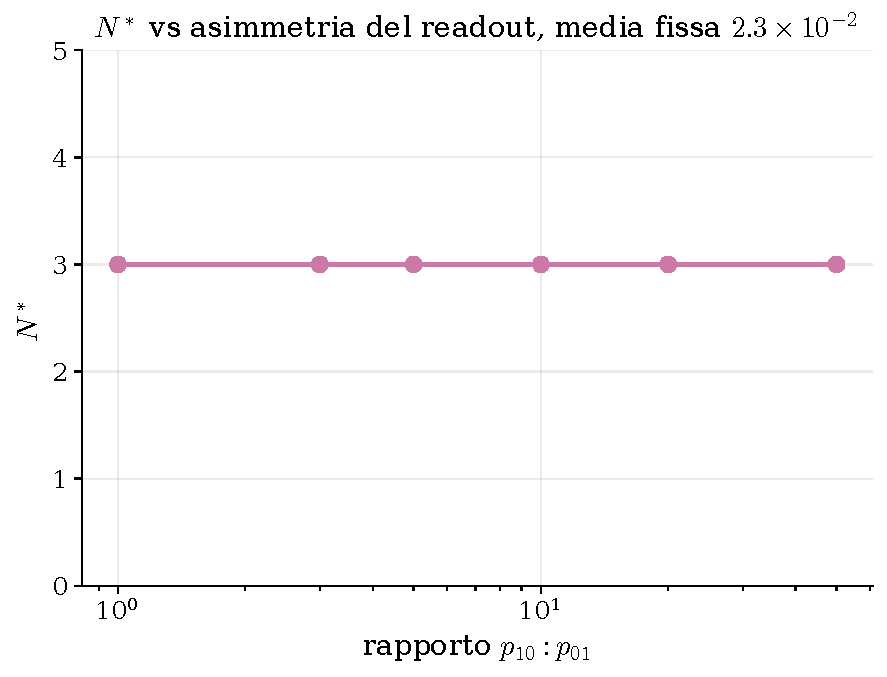
\includegraphics[width=0.62\textwidth]{figure/fig_Nstar_vs_rapporto_anello}
\caption{$N^*$ in funzione del rapporto $p_{10}/p_{01}$, da $1\times$ a
$50\times$ --- ben oltre il range realistico osservato su hardware IBM
(tipicamente $2$--$3.5\times$), stessa media $2.3\times10^{-2}$.}
\end{figure}
\FloatBarrier

$N^*=3$ su tutti e sei i rapporti testati ($1,3,5,10,20,50\times$),
verificato a shot finiti su ciascun punto --- non solo al riferimento.

\section{Perché non ha ceduto nemmeno a rapporti estremi}

Stessa lettura del dimero: $N^*$ è definito dal massimo di una curva
$|C(N)|$ già ripida attorno al suo picco (Documento 8); una traslazione
costante ($\beta$ nella formula) sposta la curva intera, ma raramente
abbastanza da spostare la posizione del suo massimo, finché $\alpha>0$
(cioè finché $p_{01}+p_{10}<1$, sempre vero nel range fisico qui
esplorato).

\section{Considerazioni}

Estensione chiusa senza sorprese, a differenza dell'estensione del
Documento 10: nessun ostacolo concettuale confermato (il registro più
grande non tocca la correzione), nessun comportamento anomalo. L'unico
punto che richiedeva attenzione --- la diversa convenzione dei qubit
dell'ancilla --- è stato identificato e verificato esplicitamente prima
di scrivere il codice, non scoperto a posteriori da un risultato
sbagliato.

\section{Dove chiude la Parte 2 sull'anello}

Con questo documento si chiudono, sull'anello, tutti e cinque gli stadi
più le due estensioni facoltative --- lo stesso livello di completezza già
raggiunto sul dimero. Filoni possibili per il seguito, non affrontati qui:
la stessa Parte 2 sulla topologia a catena aperta (Parte 1 già completa,
Parte 2 mai iniziata), o un secondo punto di lavoro per l'estensione del
Documento 10, per verificarne la generalità come già fatto sul dimero.

\end{document}
